\begin{table}[h]
\centering
\begin{tabular}{|c|l|}
\hline
Name & Implementation \\ \hline 
$I$ equals $J$ & if $s_i = s_j \wedge e_i = e_j $ \\
$I$ starts $J$ & if $s_i = s_j \wedge e_i < e_j $ \\
$I$ started by $J$ & if $s_i = s_j \wedge e_i > e_j $ \\
$I$ finishes $J$ & if $s_i > s_j \wedge e_i = e_j $ \\
$I$ finished by $J$ & if $s_i < s_j \wedge e_i = e_j $ \\
$I$ meets $J$ & if $e_i = s_j $ \\
$I$ met by $J$ & if $s_i = e_j $ \\
$I$ overlaps $J$ & if $s_i < s_j \wedge e_i < e_j \wedge e_i > s_j $ \\
$I$ overlapped by $J$ & if $s_i > s_j \wedge e_j < e_i \wedge s_i < e_j  $ \\
$I$ during $J$ & if $s_i > s_j \wedge e_i < e_j $ \\
$I$ contains $J$ & if $  s_i < s_j \wedge e_i > e_j$ \\
$I$ before $J$ & if $e_i < s_j $ \\
$I$ after $J$ & if $s_i > e_j $ \\
\hline
\end{tabular}
\caption{Allen's relations represented in the framework. $I = \left[s_i, e_i\right]$, $J=  \left[s_j, e_j\right]$}
\label{tab:allen-relations}
\end{table}


\begin{figure}[h]
   \centering
   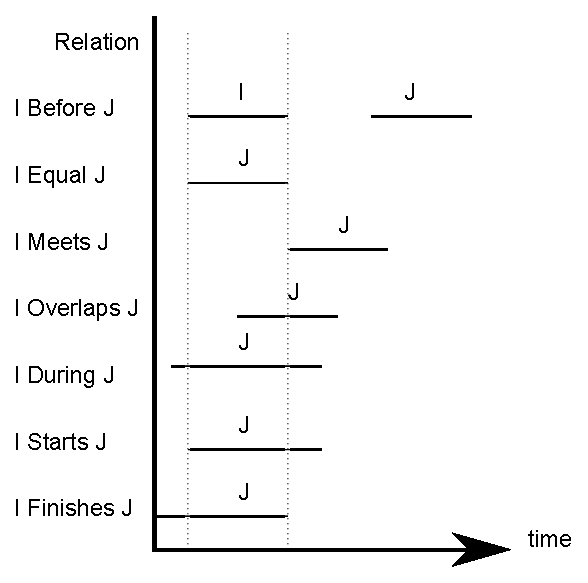
\includegraphics[width=0.8\columnwidth]{graphs/allen.eps}
   \caption{The Allen relationships between two crisp intervals $I$ and $J$.  }
   \label{fig:allen-relationships}
 \end{figure}
